%\documentclass[11pt, a4paper,dalthesis]{report}    % final
%\documentclass[11pt,a4paper,dalthesis]{report}
%\documentclass[11pt,a4paper,dalthesis]{book}

\documentclass[11pt,a4paper,titlepage,oneside,openany]{article}

\pagestyle{plain}
%\renewcommand{\baselinestretch}{1.7}

\usepackage{setspace}
%\singlespacing
%\onehalfspacing
%\doublespacing
%\setstretch{1.1}

\usepackage{amsmath}
\usepackage{amssymb}
\usepackage{amsthm}
\usepackage{multicol}

\usepackage[margin=3cm]{geometry}
\usepackage{graphicx,psfrag}%\usepackage{hyperref}
\usepackage[small]{caption}
\usepackage{subfig}

\usepackage{algorithm}
\usepackage{algorithmic}
\newcommand{\theHalgorithm}{\arabic{algorithm}}

\usepackage{varioref} %NB: FIGURE LABELS MUST ALWAYS COME DIRECTLY AFTER CAPTION!!!
%\newcommand{\vref}{\ref}

\usepackage{index}
\makeindex
\newindex{sym}{adx}{and}{Symbol Index}
%\newcommand{\symindex}{\index[sym]}
%\newcommand{\symindex}[1]{\index[sym]{#1}\hfill}
\newcommand{\symindex}[1]{\index[sym]{#1}}

%\usepackage[breaklinks,dvips]{hyperref}%Always put after varioref, or you'll get nested section headings
%Make sure this is after index package too!
%\hypersetup{colorlinks=false,breaklinks=true}
%\hypersetup{colorlinks=false,breaklinks=true,pdfborder={0 0 0.15}}


%\usepackage{breakurl}

\graphicspath{{./images/}}

\usepackage[subfigure]{tocloft}%For table of contents
\setlength{\cftfignumwidth}{3em}

\input{longdiv}
\usepackage{wrapfig}


%\usepackage{index}
%\makeindex
%\usepackage{makeidx}

%\usepackage{lscape}
\usepackage{pdflscape}
\usepackage{multicol}

\usepackage[utf8]{inputenc}

%\usepackage{fullpage}

%Compulsory packages for the PhD in UL:
%\usepackage{UL Thesis}
\usepackage{natbib}

%\numberwithin{equation}{section}
\numberwithin{equation}{section}
\numberwithin{algorithm}{section}
\numberwithin{figure}{section}
\numberwithin{table}{section}
%\newcommand{\vec}[1]{\ensuremath{\math{#1}}}

%\linespread{1.6} %for double line spacing

\usepackage{afterpage}%fingers crossed

\newtheorem{thm}{Theorem}[section]
\newtheorem{defin}{Definition}[section]
\newtheorem{cor}[thm]{Corollary}
\newtheorem{lem}[thm]{Lemma}

%\newcommand{\dbar}{{\mkern+3mu\mathchar'26\mkern-12mu d}}
\newcommand{\dbar}{{\mkern+3mu\mathchar'26\mkern-12mud}}

\newcommand{\bbSigma}{{\mkern+8mu\mathsf{\Sigma}\mkern-9mu{\Sigma}}}
\newcommand{\thrfor}{{\Rightarrow}}

\newcommand{\mb}{\mathbb}
\newcommand{\bx}{\vec{x}}
\newcommand{\bxi}{\boldsymbol{\xi}}
\newcommand{\bdeta}{\boldsymbol{\eta}}
\newcommand{\bldeta}{\boldsymbol{\eta}}
\newcommand{\bgamma}{\boldsymbol{\gamma}}
\newcommand{\bTheta}{\boldsymbol{\Theta}}
\newcommand{\balpha}{\boldsymbol{\alpha}}
\newcommand{\bmu}{\boldsymbol{\mu}}
\newcommand{\bnu}{\boldsymbol{\nu}}
\newcommand{\bsigma}{\boldsymbol{\sigma}}
\newcommand{\bdiff}{\boldsymbol{\partial}}

\newcommand{\tomega}{\widetilde{\omega}}
\newcommand{\tbdeta}{\widetilde{\bdeta}}
\newcommand{\tbxi}{\widetilde{\bxi}}



\newcommand{\wv}{\vec{w}}

\newcommand{\ie}{i.e. }
\newcommand{\eg}{e.g. }
\newcommand{\etc}{etc}

\newcommand{\viceversa}{vice versa}
\newcommand{\FT}{\mathcal{F}}
\newcommand{\IFT}{\mathcal{F}^{-1}}
%\renewcommand{\vec}[1]{\boldsymbol{#1}}
\renewcommand{\vec}[1]{\mathbf{#1}}
\newcommand{\anged}[1]{\langle #1 \rangle}
\newcommand{\grv}[1]{\grave{#1}}
\newcommand{\asinh}{\sinh^{-1}}

\newcommand{\sgn}{\text{sgn}}
\newcommand{\morm}[1]{|\det #1 |}

\newcommand{\galpha}{\grv{\alpha}}
\newcommand{\gbeta}{\grv{\beta}}
%\newcommand{\rnlessO}{\mb{R}^n \setminus \vec{0}}
\usepackage{listings}
\usepackage{arydshln}

\interfootnotelinepenalty=10000

\newcommand{\sectionline}{%
	\nointerlineskip \vspace{\baselineskip}%
	\hspace{\fill}\rule{0.5\linewidth}{.7pt}\hspace{\fill}%
	\par\nointerlineskip \vspace{\baselineskip}
}

\renewcommand{\labelenumii}{\roman{enumii})}

\begin{document}
	
	\begin{center}
		\textbf{Tutorial Sheet 6}
	\end{center}
	
	\begin{enumerate}
		\item For the vectors given below, evaluate the following expressions where it is possible.
		\begin{equation*}
		\vec{u}=\left[ \begin{array}{c} 1 \\ 2 \\ 3 \end{array}\right],
		\vec{v}=\left[ \begin{array}{c} -1 \\ 0 \\ 4 \end{array}\right],
		\vec{x}=\left[ \begin{array}{c} 3 \\ 4 \end{array}\right],
		\vec{y}=\left[ \begin{array}{c} -4 \\ 3 \end{array}\right],
		\vec{w}=\left[ \begin{array}{c} 1 \\ 0\\ 2 \\ -5 \end{array}\right],
		\vec{z}=\left[ \begin{array}{c} 2 \\ 2 \\ 2 \\ 3 \end{array}\right]
		\end{equation*}
		\begin{multicols}{3}
			\begin{enumerate}
				\item $2\vec{u} + 3\vec{v}$
				\item $3\vec{u} - \vec{v}$
				\item $\vec{x} + 3\vec{v}$
				\item $2\vec{z} - \vec{w}$
				\item $\vec{u}+\vec{x}$
				\item $\vec{v}+\vec{w}$
				\item $\vec{u}\cdot \vec{v}$
				\item $\left(2\vec{u}\right)\cdot \left(3\vec{v}\right)$
				\item $\vec{x}\cdot \vec{y}$
				\item $\vec{w} \cdot \vec{z}$
				\item $\vec{w} \cdot (\vec{z}+\vec{w})$
				\item $|\vec{x}|$
				\item $|\vec{w}|$
				\item $|\vec{y}|+|\vec{w}|$
			\end{enumerate}
		\end{multicols}
		
		\item
		Calculate the angles between the pairs $\vec{u},\vec{v}$, $\vec{x},\vec{y}$, and $\vec{w},\vec{z}$ from the previous question. Give your answers in both radians and degrees.
		
		\item
		For the matrices below, evaluate the following expressions where it is possible.
		\begin{equation*}
		A=\left[ \begin{array}{cc} 1  & 2 \\ 3 & 4 \end{array}\right],
		B=\left[ \begin{array}{cc} -2  & 0 \\ 1 & -7 \end{array}\right],
		C=\left[ \begin{array}{ccc} 3  & 2 & -2 \\ 4 & 8 & 2 \end{array}\right],
		D=\left[ \begin{array}{ccc} 3  & 2 & -2 \\ 4 & 8 & 2 \end{array}\right],
		\end{equation*}
		\begin{equation*}
		E=\left[ \begin{array}{ccc} 1  & 2 & 3 \\ 4 & 5 & 6 \\ 7 & 8 & 9 \end{array}\right],
		F=\left[ \begin{array}{ccc} -1  & 0 & 2 \\ 3 & 4 & 1 \\  3 & 1 & 0 \end{array}\right],
		\end{equation*}
		%-------------------%
		\begin{equation*}
		G=\left[ \begin{array}{cc}3 & 4 \\1 & 2 \\2 &-1 \\ \end{array}\right],
		H=\left[ \begin{array}{ccc}3 & 4 & 3\\1 & 2 & 2\\ \end{array}\right],
		I=\left[ \begin{array}{ccc}2 & 2 & 1\\ \end{array}\right],
		\end{equation*}
		%-------------------%
		\begin{equation*}
		J=\left[ \begin{array}{c}
		3\\
		1\\
		1\\ \end{array}\right],
		K=\left[ \begin{array}{ccc}
		2 & 1 & 3\\1 & 2 & 2\\2 & 1 & 0\\\end{array}\right], 
		\end{equation*}
		%-------------------------------%
		\begin{multicols}{3}
			\begin{enumerate}
				\item $2A+3B$
				\item $3C-D$
				\item $8A+4C$
				\item $2000A+3000B$
				\item $E-F$
				\item $A\vec{x}$
				\item $B\vec{x}$
				\item $A\vec{y}+B\vec{x}$
				\item $A\vec{u}$
				\item $C\vec{x}$
				\item $C\vec{w}$
				\item $E\vec{u}$
				\item $E\vec{w}-\vec{F}\vec{w}$
				
			\end{enumerate}
		\end{multicols}
		
	\end{enumerate}
\end{document}
\pagebreak

\begin{center}
	\textbf{Tutorial Sheet 7}
\end{center}

\begin{enumerate}
	\item
	For each of the following systems of linear equations, write down the corresponding coefficient matrix $A$, vector of unknowns $\vec{x}$, and vector of right hand sides $\vec{b}$ so that the system can be expressed in the form $A\vec{x}=\vec{b}$
	\begin{multicols}{3}
		\begin{enumerate}
			\item
			\begin{align*}
			2x+3y&=1\\
			5x+7y&=3
			\end{align*}
			\item\begin{align*}
			2x+3y+4z&=1\\
			x-2y+2z&=7\\
			3x+2y+z&=0.2
			\end{align*}
			\item
			\begin{align*}
			3x+y+z&=1\\
			y+4z&=-4\\
			x-y&=2
			\end{align*}
		\end{enumerate}
	\end{multicols}
	\item
\end{enumerate}
%\begin{wrapfigure}{r}{0.5\textwidth}
%    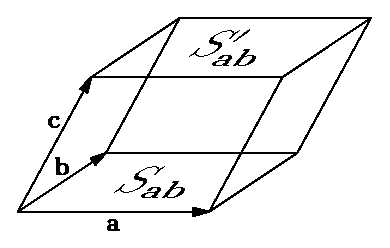
\includegraphics[width=0.5\textwidth]{par3_tut}
%    \vspace{-5em}
%\end{wrapfigure}

Let the vectors $\vec{a},\vec{b},\vec{c}$ be given by
\begin{equation*}
\vec{a}=\left[ \begin{array}{c} 2 \\ 0 \\ 0 \end{array}\right],
\vec{b}=\left[ \begin{array}{c} 2 \\ 1 \\ 0 \end{array}\right],
\vec{c}=\left[ \begin{array}{c} 2 \\ 0 \\ 1 \end{array}\right]
\end{equation*}
These vectors span a three dimensional parallelopiped as shown in the figure to the right.

\begin{enumerate}
	\renewcommand{\theenumi}{\roman{enumi})}
	\renewcommand{\labelenumi}{\theenumi}
	{\setlength\itemindent{3em} \item
		Find the area of the parallelogram $S_{\vec{a}\vec{b}}$ which is spanned by the vectors $\vec{a}$ and $\vec{b}$. Hence state the area of the parallelogram $S_{\vec{a}\vec{b}}'$ on the opposite side of the parrallelopiped.}
	{\setlength\itemindent{3em} \item
		Find the areas of the parallelograms $S_{\vec{b}\vec{c}}$ and $S_{\vec{a}\vec{c}}$ spanned by the relevant pairs of vectors and hence find the total surface area of the parrallelopiped.}
	{\setlength\itemindent{3em} \item
		Find the signed volume of the parrallelopiped.}
\end{enumerate}

\begin{enumerate}
	\setcounter{enumi}{2}
	\item
	Rotate the point $\vec{x}=\left[ \begin{array}{c} 1 \\ 3 \end{array}\right]$ anti-clockwise $\frac{\pi}{4}$ radians about the point $\vec{p}=\left[ \begin{array}{c} 2 \\ 2 \end{array}\right]$.
	\item
	Rotate the line segment with endpoints $\vec{x}=\left[ \begin{array}{c} 1 \\ 3 \end{array}\right]$ and $\vec{y}=\left[ \begin{array}{c} 3 \\ 3 \end{array}\right]$ anti-clockwise $\frac{\pi}{2}$ radians about the point $\vec{p}=\left[ \begin{array}{c} 2 \\ 2 \end{array}\right]$. Give the new endpoints $\vec{x}'$ and $\vec{y}'$ of the rotated line segment.
\end{enumerate}

\section{Counting methods and probability}

Chapter 5
Systems of linear equations and
matrices
Essential reading
M&B Sections 6.1, 6.2. Only part of this chapter is covered in Epp (Section 11.8)
Keywords



Systems of linear equations; Gaussian elimination. Matrix algebra.
It often happens that information has to be stored in a list or a table.
Matrices are a convenient way of representing such data, as you
have already experienced with the incidence matrix of graphs and
digraphs. We thus study the basics of matrix algebra in this chapter.



We shall also see that a system of 7L linear equations in 7L unknowns
can be conveniently expressed in the form of a matrix equation. The
equations in this form can be solved in an algorithmic manner. The
method is suitable for programming into a computer, which
distinguishes it from the methods for solving equations you learnt in
school. The algorithm for solving systems of linear equations is
known as Gaussian Elimination.



Systems of linear equations
Learning objectives for this section
I Recognizing linear and non-linear equations
I Writing down the augmented matrix of a system of linear equations
I Using Gaussian elimination to reduce a matrix to row echelon form
I Using Gaussian elimination and back substitution to lind all solutions to a system
of linear equations
Definition 5.1 A linear equation in n. unknowns 1-1,1»; . . . ,1.-,L is an
equation of the form
(1111 + agar; + . . . + awmn = b





ClS102 Mathematics ior computing volume 2
where (11,112. . . . , an and b are given real numbers.
Example 5.1 The equation
, ,, _ 1
.£1+2£F2’l.3 — E
is a linear equation.
The equations $112 = 3 or  + 1:2 = 4 or log(r1) + .'I?2 = 7 are not
linear.
Definition 5.2 A system of linear equations in n. unknowns
r1‘w2_ . . . ,1~,, is a collection of one or more linear equations involving
the same unknowns. A solutionfor this system is an assignment of
real numbers .11 : kl, ac; = k2, . . . ,;1c,,, = kn which satisfies each of the
equations in the system. To solve the system we want to find all the
solutions to the system.



Example 5.2 A system of linear equations and its solution
Consider the following system of two equations in two unknowns.
3.r1 + 612 = 60 (5.1)
211 — 1'2 = 10. (5.2)
Then %>< Equation (5.1) is
001 + 2172 = Z0. (5.3)
Now Equation (5.2) — 2>< Equation (5.3) gives
—5.rZ = -30.
Therefore
.rg = 6.
Substituting back into Equation (5.3) gives
av1=2O—2av2 =20—12=8.
So the only solution to this system is $1 = 8 and 12 = 6.
We can solve a system of m equations with n unknowns using a
method similar to the one of Example 5.2 by first reducing to m — 1
equations with n — 1 unknowns, then m — 2 equations with n — 2
unknowns, and so on. To describe accurately the general procedure
we use matrices.
Definition 5.3 An m. >< n matrix is a rectangular array of real numbers
with m rows and n columns.
01 -2
A1< >
_§ 3 5



We shall usually use upper case letters such as A, B, X to represent
matrices. The only exception being for matrices with just one row or
one column which we represent by bold face letters, such as b. Note
that other books may use a different notation. Some authors use
overlined or underlined letters, such as h or Q, or even underlined
bold face letters like I3 for matrices with one row/column.
74
Example 5.3 The matrix
is a 2 >< 3 matrix.





We write A = (aw-) to mean that the entry in the ith row and the jth
column of A is labelled a.,_,. Sometimes we also use the notation
A(i,j) for the entry in the ith row and the jth column of A.
Example 5.3 (cont.) In this matrix 0.17; = 1 and 11.2,] = —%.
Definition 5.4 We can write a system of m equations in n unknowns as:
M1961 + ll1,2Jv2 +  + 111.1%" = bi
(Z2111 + (Lgyglljg +  + (L2Yn.’l‘n = 122
um.1-T1 + amzwz +  + ammwn = bm
where am and b,-I are given real numbersfor 1 § 2} § m and 1 § j § 11..



The matrix of coeflicients for this system is the m >< n matrix A in
which the entry in the ith row and jth column is the coeflicient of the
unknown rj in the ith equation of the system. Thus, using the above
representation for the system, we have A = (aw-), that is
111.1 (11.2  I11,"
@2.1 112.2  dz,"
A = _
am am;  am.
The augmented matrix for this system is the m >< (n + 1) matrix
(A : b) which we get by adding the extra column
“(ii
to the right of A, that is the augmented matrixfor the system is
(11.1 111,2  aim I bl
112.1 <l2,2  I12.” I 52
(AIb)= . .
u’m,1 am;  a’m_7l I bm



Example 5.4 The augmented matrix of a system oi linear equations
For the system of equations of Example 5.2 we have the matrix of
coefficients
3 6
A e ( 2 -1 >
and the augmented matrix
_i z :2)
We shall solve the system of equations of Example 5.2 by using the
following three operations on the rows of the augmented matrix
(A : b) rather than working with the equations (5.1) and (5.2).

\begin{itemize}
	\item Interchange two rows.
	\item Multiply a row by a non-Zero real number.
	\item Add multiples of one row to another row.
	
	
	
	
	
	C|S102 Mathematics ior computing volume 2
	To describe which operation we are using we denote the first and
	second rows of (A : b) by R1 and R2 respectively We first multiply
	R1 by 1/3, so R1 := %R1:
	1 2 : 20
	2 —1 : 10 '
	We next subtract twice R1 from R2, so R2 := R2 — 2R1:
	1 2 : 20
	O —5 : ~30
	From the final augmented matrix we can read off the solution as
	follows:
	R2 :> —5a?2 = -30 :> r2 = 6.
	Now substituting this into the equation corresponding to R1 we get
	R1 =>x1+2m2=20=>m1 =20—2x2=20—(2><6)=8.
	You can check that these values for $1, r2 satisfy both the equations
	of Example 5.2 by substituting into the equations:
	3 - 8 + 6 - 6 = 60
	2 1 8 — 6 = 1O
	
	
	
	Example 5.5 We now solve the system
	1'2 + 2x3 = 3
	ZT1 + 3.102 : 1
	11 + $2 — av; = 1.
	
	
	
	The augmented matrix is
	O l 2 : 3
	(A:b)= Z 3 O : 1
	1 1 *1 : 1
	Like the previous example we number the rows of the augmented
	matrix R1, R2 and R3. We first interchange the first row (R1) with
	the third row (R3) to bring a one into the upper left hand corner of
	the augmented matrix, that is R1 <-> R3:
	1 1 —1
	O 1 2
	
	
	
	We next subtract twice the first row from the second row so that all
	entries in the first column, below the first entry, become equal to
	zero, that is R2 z: R2 — 2R1:
	< _1 )
	Finally, we subtract the second row from the third row so that the
	entry in the second column, below the second entry, becomes equal
	to zero. R3 2: R3 — R2:
	co»; N
	)—\P—\Pi D)
	NN O
	www “H”
	V
	@@>—\
	Ow»-I
	ON
	>J>>-
	Li
	—1: 1
	76
	
	
	
	
	
	Systems of linear equations
	The system of equations corresponding to the final augmented
	matrix is
	1'1 + at; — x3 = 1
	O11 + 1'2 + 213 = -1
	OT] + Om; + 0.733 : 4.
	Now R3 :> Om + 0.12 + O13 = 4. Since we cannot have
	O11 + Or; + OJE3 = 4, there are no solutions to this system of
	equations.
	
	
	
	Example 5.6 We solve a system with the same matrix of coefficients as
	in Example 5.5, but a different column b.
	IE2 + 2173 = 3
	211 + 31"; = 1
	11 + 1'2 — 13 = -1
	The augmented matrix is
	>—\I\7©
	>—\ua>~
	>—l(Dl\7
	>—\>—\UJ
	(A:b)=
	Proceeding as in Example 5.5:
	R1 <—> R3
	1 1 —1 : —
	@l\J
	wt»
	NO
	UJ>—\>—\
	R2:=R2—2R1
	@@>4
	»-1»-I
	NN
	wo-vii
	1 -1: —
	R3:=R3—R;
	@@»—\
	Qvd
	QN
	©UJ>—\
	1—1:—
	
	
	The system of equations corresponding to the final augmented
	matrix is
	1'1 + 1'; — 1'3 = —1
	$2 + 2.13 = 3
	0 = O.
	Note that the third equation holds trivially for all values of J?1,.7?2. $3,
	so we have found that the original system is equivalent to a system
	of two linear equations in three unknowns. When there are less
	equations than unknowns, the system has either infinitely many
	solutions or no solution at all. This system has infinitely many
	solutions.
	
	
	
	We can write down the general solution by working our way
	backwards through the system of equations corresponding to the
	final augmented matrix:
	R2:m2+2x3=3.
	So
	T2 = 3 — ZI3.
	We let  = r where 1- is any real number. Then $2 = 3 — Zr. Now
	R1¢z1+.r;—av3=—1.
	77
	
	
	
	ClS102 Mathematics lor computing volume 2
	So
	$1=*1~m2+:n3=~1~(3~Zr)+7‘=~4-l-31".
	Thus the general solution is 1:1 = —4 + 3r, 1:2 = 3 — 21" and $3 = r,
	where r E R. We have infinitely many solutions as we get a different
	solution for ml , 1;, 41:3 for each real number r.
	Gaussian elimination
	The algorithm we used to solve the systems of linear equations
	given in Examples 5.4, 5.5 and 5.6 is called Gaussian elimination.
	It gives a general method for solving all such systems.
	
	
	
	The Gaussian elimination algorithm
	We start with the augmented matrix (A : b) for the system. We then
	reduce (A : b) to a ‘simpler’ augmented matrix (A* : b*) by using the
	following steps:
	Step1 Choose the leftmost column of (A : b) which contains a
	non-zero entry. Call it the pivot column.
	Step 2 Interchange the first row with another row, if necessary,
	so that the top entry in the pivot column is non-Zero. Call
	this entry the pivot.
	
	
	Step 3 Multiply the first row by a suitable real number so that
	the pivot becomes equal to 1.
	Step 4 Subtract multiples of the first row from the other rows so
	that all entries in the pivot column, below the pivot entry,
	become equal to zero.
	
	
	
	Step 5 Now disregard the first row and return to step 1 with the
	resulting smaller matrix.
	Step 6 Stop either when there are no more rows or all columns
	contain only zeros.
	
	
	
	The output of this algorithm will be an augmented matrix with a
	very simple type of structure. To describe this structure precisely we
	need one further definition.
	Definition 5.5 Let M be an m >< n matrix Then an entry of M is said to
	be a leading entry if it is the first non-zero entvfy in some row.
	Example 5.7 The following matrix M has three leading entries, which
	are given in bold face.
	Ill = (
	
	
	
	Row 4 has no leading entry as it consists entirely of entries zero.
	<3<3Or—l
	@I§©©
	CDIQUOIQ
	<3O‘\U‘|(.|J
	The output from Gaussian elimination is an augmented matrix with
	the four properties listed below:
	P1 All rows which consist entirely of zeros occur at the bottom.
	P2 All leading entries are equal to 1.
	78
	
	
	
	P3 If a column contains a leading entry then all entries in that
	column below the leading entry are zero.
	P4 In any two consecutive non-zero rows, the leading entry in the
	upper row occurs to the left of the leading entry in the lower
	row.
	
	
	
	Definition 5.6 A matrix which satisfies properties P1 to P4 is said to be
	in row echelon form.
	Given an augmented matrix in row echelon form (A* : b*), we can
	easily write down the solution to the corresponding system of
	equations. There are three possible cases:
	Case 1: Some leading entry occurs in the final column b*.
	In this case we deduce that there is no solution. For example:
	©®>—\
	@@|\)
	@@>—\
	O>—\v|>
	R; => Owl + 0372 + 0703 = 1 => No solution.
	Case 2: The final column does not contain a leading entry but all
	other columns do contain a leading entry.
	
	
	
	In this case the system has a unique solution. We obtain this
	solution by the process of back substitution: we use the final
	non-zero row to determine the unknown, av”, corresponding to
	the last column of A*, then use the second to last row and
	substitute for ac” to determine .1:,,_1 and so on. For example:
	@@>—\
	@>dI\J
	>-I >—\
	Ull\7>—\
	_1-
	R3:>.r3:5.
	R2=>z2=2+.1:3=2+5=7.
	R1=>m1=—1—Zx2—x3=—1—l4—5=—2O.
	So the unique solution is 11 = —2O,z2 = 7,13 =5.
	Case 3: The final column and some other columns do not contain
	leading entries.
	
	
	
	In this case the system has infinitely many solutions. We set the
	unknowns corresponding to the columns of A* which do not
	contain leading entries equal to arbitrary real numbers, then use
	back substitution to solve for the remaining unknowns. For
	example:
	@@>—'
	@©l\l
	QQUJ
	Qré
	(DUl>—\
	-1
	R1 Q 1'4 = 3.
	We can choose .203 and 12 freely because columns 3 and 2 of the
	augmented matrix in row echelon form contain no leading
	entries, so set 11:3 = r where r E R and ac; = s where s E IR.
	R1¢11=1—2m2 +ar4=1—2s—3r+3=4—2s—3r.
	So the general solution is ml = 4 — 25 — 3r, 1:2 = s, 1:3 = r, $4 = 3,
	forvgs E R.
	Systems of linear equations
	%- 79

%-------------------------------------------------------%
\frame{
	\frametitle{Basic Operations with Matrices }
	
	\begin{itemize}
		\item Addition of Matrices
		\item Transpose of a Matrix
		\item Adding and Subtracting Matrices
		\item Scalar Multiplication
	\end{itemize}
}

%-------------------------------------------------------%
\frame{
	
	\frametitle{Matrix Multiplication}
	{
		\huge
		\textbf{
			\[ \left(
			\begin{array}{cc}
			a & b \\
			c & d \\
			\end{array}
			\right) \times \left(
			\begin{array}{cc}
			u & v \\
			w & x \\
			\end{array}
			\right)
			\]
		}
	}
	
	
}
%-------------------------------------------------------%
\frame{
	
	
	{
		\huge
		\textbf{
			\[ \left(
			\begin{array}{cc}
			a & b \\
			c & d \\
			\end{array}
			\right) \times \left(
			\begin{array}{cc}
			u & v \\
			w & x \\
			\end{array}
			\right)
			\]
		}
	}
	\bigskip
	{
		\huge
		\textbf{
			\[ \left(
			\begin{array}{cc}
			3 & 1 \\
			2 & 4 \\
			\end{array}
			\right) \times \left(
			\begin{array}{cc}
			2 & 5 \\
			4 & 1 \\
			\end{array}
			\right)
			\]
		}
	}
}

%-------------------------------------------------------%
\frame{
	\frametitle{Matrix Multiplication}
	
	{\huge
		\textbf{
			\[ \left(
			\begin{array}{cc}
			\underline{\alert{a}}& \underline{\alert{b}} \\
			c & d \\
			\end{array}
			\right) \times \left(
			\begin{array}{cc}
			u & v \\
			w & x \\
			\end{array}
			\right)
			\]
		} % End Bold
	} % End Huge
} % End Frame

%-------------------------------------------------------%
\frame{
	\frametitle{Matrix Multiplication}
	
	{\huge
		\textbf{
			\[ \left(
			\begin{array}{cc}
			\alert{a} & \alert{b} \\
			c & d \\
			\end{array}
			\right) \times \left(
			\begin{array}{cc}
			\underline{\textcolor{green}{u}} & v \\
			\underline{\textcolor{green}{w}} & x \\
			\end{array}
			\right)
			\]
		}
	}
}
%-------------------------------------------------------%
\frame{
	\frametitle{Matrix Multiplication}
	
	{\huge
		\textbf{
			\[ \left(
			\begin{array}{cc}
			\alert{a} & \alert{b} \\
			c & d \\
			\end{array}
			\right) \times \left(
			\begin{array}{cc}
			\textcolor{green}{u} & v \\
			\textcolor{green}{w} & x \\
			\end{array}
			\right)
			\]
		}
		\textbf{
			\[ = \left(
			\begin{array}{cc}
			\alert{a}\textcolor{green}{u} + \alert{b}\textcolor{green}{w}& \ldots \ldots\\
			\ldots \ldots & \ldots \ldots \\
			\end{array}
			\right) 
			\]
		}
	}
}
%-------------------------------------------------------%
\frame{
	\frametitle{Basic Operations with Matrices  }
	
	
	\textbf{Transpose of a Matrix}
	\begin{itemize}
		
		\item The transpose of a matrix is transformation of that matrix when all the rows are arranged into columns and columns arranged by rows.
		\item The transpose of a matrix $A$ is usually denoted $A^{T}$ or $A^{\prime}$.
		\item The relevant \texttt{R} function is \texttt{t()}.
	\end{itemize}
}

\end{document}
%-------------------------------------------------------%
\frame{
	\frametitle{Sample Space (2)}
	Consider a random experiment in which a coin is tossed once, and a number between 1 and 4 is selected at random.
	Write out the sample space $S$ for this experiment.
	
	\bigskip
	
	\[ S = \{(H,1),(H,2),(H,3),(H,4),(T,1),(T,2),(T,3),(T,4)\} \]
	
	( $H$ and $T$ denoted `Heads' and `Tails' respectively. )
	
}
%-------------------------------------------------------%
\frame{
	\frametitle{Contingency Tables}
	Suppose there are 100 students in a first year college intake.  \begin{itemize} \item 44 are male and are studying computer science, \item 18 are male and studying statistics \item 16 are female and studying computer science, \item 22 are female and studying statistics. \end{itemize}
	\bigskip
	We assign the names $M$, $F$, $C$ and $S$ to the events that a student, randomly selected from this group, is male, female, studying computer science, and studying statistics respectively.
}
%-------------------------------------------------------%
\frame{
	\frametitle{Contingency Tables}
	The most effective way to handle this data is to draw up a table. We call this a \textbf{\emph{contingency table}}.
	\\A contingency table is a table in which all possible events (or outcomes) for one variable are listed as
	row headings, all possible events for a second variable are listed as column headings, and the value entered in
	each cell of the table is the frequency of each joint occurrence.
	
	
	\begin{center}
		\begin{tabular}{|c|c|c|c|}
			\hline
			% after \\: \hline or \cline{col1-col2} \cline{col3-col4} ...
			& C & S & Total \\ \hline
			M & 44 & 18 & 62 \\ \hline
			F & 16 & 22 & 38 \\ \hline
			Total & 60 & 40 & 100 \\ \hline
		\end{tabular}
	\end{center}
	
}
%-------------------------------------------------------%
\frame{
	\frametitle{Contingency Tables}
	It is now easy to deduce the probabilities of the respective events, by looking at the totals for each row and column.
	\begin{itemize}
		\item P(C) = 60/100 = 0.60
		\item P(S) = 40/100 = 0.40
		\item P(M) = 62/100 = 0.62
		\item P(F) = 38/100 = 0.38
	\end{itemize}
	\textbf{Remark:}\\
	The information we were originally given can also be expressed as:
	\begin{itemize}
		\item $P(C \cap M) = 44/100 = 0.44$
		\item $P(C \cap F) = 16/100 = 0.16$
		\item $P(S \cap M) = 18/100 = 0.18$
		\item $P(S \cap F) = 22/100 = 0.22$
	\end{itemize}
}

%-------------------------------------------------------%
\frame{
	\frametitle{Conditional Probability (1)}
	
	The definition of conditional probability:
	\[ P(A|B) = \frac{P(A \cap B)}{P(B)} \]
	
	\begin{itemize}
		\item $P(B)$ Probability of event B.
		\item [ $P(A)$ Probability of event A. ]
		\item $P(A|B)$ Probability of event A given that B has occurred.
		\item $P(A \cap B)$ Joint Probability of event A and event B.
		\item Will be given tomorrow.
	\end{itemize}
	
}


%-------------------------------------------------------%
\frame{
	\frametitle{Conditional Probabilities (2)}
	
	Compute the following:
	\begin{enumerate}
		\item $P(C|M)$ : Probability that a student is a computer science student, given that he is male.
		\item $P(S|M)$ : Probability that a student studies statistics, given that he is male.
		\item $P(F|S)$ : Probability that a student is female, given that she studies statistics.
	\end{enumerate}
	
}
%-------------------------------------------------------%
\frame{
	\frametitle{Conditional Probabilities (3)}
	
	\textbf{Part 1)} Probability that a student is a computer science student, given that he is male.
	\[ P(C|M) = \frac{P(C \cap M)}{P(M)}  = \frac{0.44}{0.62} = 0.71 \]
	\textbf{Part 2)} Probability that a student studies statistics, given that he is male.
	\[ P(S|M) = \frac{P(S \cap M)}{P(M)}  = \frac{0.18}{0.62} = 0.29 \]
	
}

%-------------------------------------------------------%
\frame{
	\frametitle{Conditional Probabilities (4)}
	
	\textbf{Part 3)} Probability that a student is female, given that she studies statistics.
	\[ P(F|S) = \frac{P(F \cap S)}{P(S)}  = \frac{0.22}{0.40} = 0.55 \]
	
	
	
	
}
%------------------------------------------------------------%
\frame{
	\frametitle{Bayes' Theorem}
	Bayes' Theorem is a result that allows new information to be used to update the conditional probability of an event.
	\bigskip
	
	\[ P(A|B) = \frac{P(B|A)\times P(A)}{P(B)} \]
	
	Use this theorem to compue $P(S|F)$, the probability that a student studies statistics, given that she is female.
	
	\[ P(S|F) = \frac{P(F|S)\times P(S)}{P(F)} = {0.55 \times 0.40 \over 0.38} = 0.578\]
}

%-------------------------------------------------------%
\frame{
	\frametitle{Independent Events}
	\begin{itemize}
		\item Suppose that a man and a woman each have a pack of 52 playing cards.
		\item Each draws a card from his/her pack. Find the probability that they each draw a Queen.
		\item We define the events:
		\begin{itemize} \normalsize \item A = probability that man draws a Queen = 4/52  = 1/13
			\item B = probability that woman draws a Queen = 1/13
		\end{itemize} \item Clearly events A and B are independent so:
		\[ P(A \cap B) = 1/13 \times 1/13 = 0.005917 \]
	\end{itemize}
	
}
%---------------------------------------------------------READY---------%
\frame{
	\frametitle{Expected Value and Variance of a Random Variable}
	
	The probability distribution of a discrete random variable is be tabulated as follows
	
	\begin{center}
		\begin{tabular}{|c||c|c|c|c|c|c|}
			\hline
			$x_i$  & 1 & 2 & 3 & 4 & 5 & 6 \\\hline
			$p(x_i)$ & 2/8 & 1/8& 1/8 & 1/8& c & 1/8\\
			\hline
		\end{tabular}
	\end{center}
	
	\begin{itemize}
		\item What is the value of $c$?
		\item What is expected value and variance of the outcomes?
	\end{itemize}
}
%---------------------------------------------------------READY---------%
\frame{
	\frametitle{Expected value(1)}
	\begin{itemize}
		\item Necessarily $C =0.25 = 2/8$. \\
		\item We must compute $E(X)$ as follows \[E(X) = \sum x_i p(x_i) \]
		\item That formula is \textbf{not} given in the formulae.
	\end{itemize}
	\bigskip
	$E(X) = (1 \times {2\over8}) + (2 \times {1 \over 8}) +  \ldots + (5 \times {2 \over 8}) + (6 \times {1 \over 8})$\\\bigskip
	$E(X) = 27/8 = 3.375$\bigskip
}
%------------------------------------------------------READY------------%
\frame{
	\frametitle{Variance(1)}
	\begin{itemize}
		\item The formula for computing the variance of a discrete random variable
		
		\[ V(X) = E(X^2) - E(X)^2 \]
		
		\item This is not given in the formulae for tomorrow's exam.
		
		\item We must compute $E(X^2)$
	\end{itemize}
	
	\begin{center}
		\begin{tabular}{|c||c|c|c|c|c|c|}
			\hline
			$x_i$  & 1 & 2 & 3 & 4 & 5 & 6 \\\hline
			$x^2_i$  & 1 & 4 & 9 & 16 & 25 & 36 \\\hline
			$p(x_i)$ & 2/8 & 1/8& 1/8 & 1/8& 2/8 & 1/8\\
			\hline
		\end{tabular}
	\end{center}
}
%-----------------------------------------------------READY-------------%
\frame{
	\frametitle{Variance (2)}
	
	\begin{itemize}
		\item $E(X^2) = (1 \times {2\over8}) + (4 \times {1 \over 8}) +  \ldots + (25 \times {2 \over 8}) + (36 \times {1 \over 8})$\bigskip
		\item $E(X^2) = {117 \over 8} = 14.625$ \bigskip
		\item $V(X) = E(X^2) - E(X)^2 = 14.625 - (3.375)^2 = 3.2344$
	\end{itemize}
	\bigskip
	
}

%---------------------------------------------------%
\begin{frame}
	\frametitle{Combinations (1)}
	Combinations formula
	\[ ^{n}C_k  = {n! \over k!  \times (n-k)!} \]
	
	\begin{itemize}
		\item Remark $n! = n \times (n-1)! $
		\item 0! = 1
	\end{itemize}
\end{frame}
%---------------------------------------------------%
\begin{frame}
	\frametitle{Combinations (2)}
	Show that
	\[ ^{n}C_0  = 1 \]
	
	\textbf{Solution: }
	\[ ^{n}C_0  = {n! \over 0!  \times (n-0)!} =  {n! \over n!} = 1 \]
	
\end{frame}
%---------------------------------------------------%
\begin{frame}
	\frametitle{Combinations (3)}
	Show that
	\[ ^{n}C_1  = n \]
	
	\textbf{Solution: }
	\[ ^{n}C_1  = {n! \over 1!  \times (n-1)!} =  {n \times (n-1)! \over (n-1)!} = n \]
	
\end{frame}

%---------------------------------------------------%
\begin{frame}
	\frametitle{Combinations (4)}
	Compute $ ^{7}C_2  $\\
	
	\textbf{Solution: }
	\[ ^{7}C_2  = {7! \over 2!  \times (7-2)!} =  {7 \times 6 \times 5! \over 2! \times 5!} = {42 \over 2} =21  \]
	
\end{frame}
%---------------------------------------------------%
\begin{frame}
	\frametitle{Combinations (5)}
	Compute $ ^{11}C_1  $\\
	
	\textbf{Solution: }
	\[ ^{11}C_1  = {11! \over 1!  \times 10!} =  {11 \times 10! \over 1 \times 10!} = 11 \]
	
\end{frame}
%--------------------------------------------------------------------------------------%
\frame{
	\frametitle{Binomial Distribution (1)}
	\begin{itemize}
		\item Identify the event that can considered the `success'.
		\item (Remark : The success is usually the less likely of two complementary events.)
		\item Determine the probability of a success in a single trial $p$.
		\item Determine the number of independent trials $n$.
	\end{itemize}
	
}
%--------------------------------------------------------------------------------------%
\frame{
	\frametitle{Binomial Distribution (2)}
	The probability of exactly k successes in a binomial experiment B(n, p) is given by
	\[ P(X=k) = P(k \mbox{ successes }) = \;^nC_k  \times p^{k} \times (1-p)^{n-k}\]
	Remark: This formula will be given tomorrow.
}

%--------------------------------------------------------------------------------------%
\frame{
	\frametitle{Binomial Distribution (3)}
	
	\begin{itemize}
		
		\item Suppose we have a biased coin which yields a head only $48\%$ of the time.
		\item Is this a binomial experiment?  why?
		\item What is the probability of 4 heads in 7 throws?
	\end{itemize}
	
	
}
%--------------------------------------------------------------------------------------%
\frame{
	\frametitle{Binomial Distribution (4)}
	
	\begin{itemize}
		\item X: Number of heads thrown
		\item $n$ : number of independent trials (i.e. 7)
		\item $k$ : Number of successes (numeric value)
		\begin{itemize}
			\item Here $k$ is 4
			\item Number of failures is $n-k  =3$
		\end{itemize}
		\item $p$ : probability of a success. (i.e. 0.48)
		\item $1-p$ : probability of a failure (i.e. 0.52)
	\end{itemize}
	
}
%--------------------------------------------------------------------------------------%
\frame{
	\frametitle{Binomial Distribution (5)}
	
	\[ P(X=4) = P(4 \mbox{ successes }) = \;^7C_4  \times (0.48)^{4} \times (0.52)^{3}\]
	
	\bigskip
	
	\[ P(X=4) = 35 \times 0.05308 \times  0.14061 =  \alert{0.2612} \]
	
	Remark : must show workings.
}

%---------------------------------------------------------------------------%
\frame{
	\frametitle{Poisson Distribution(1)}
	The probability that there will be $k$ occurrences in a \textbf{unit time period} is denoted $P(X=k)$, and is computed as follows.
	\Large
	\[ P(X = k)=\frac{m^k e^{-m}}{k!} \]
	\normalsize
	This formula will be given tomorrow.
}
%---------------------------------------------------------------------------%
\frame{
	\frametitle{Poisson Distribution(2)}
	Given that there is on average 4 occurrences per day, what is the probability of one occurrences in a given day? \\ i.e. Compute $P(X=1)$ given that $m=4$
	\Large
	\[ P(X = 1)=\frac{4^1 e^{-4}}{1!} \]
	\normalsize
	
	The equation reduces to
	\[ P(X = 1)=4 \times e^{-4} = \alert{0.07326} \]
}
%---------------------------------------------------------------------------%
\frame{
	\frametitle{Poisson Distribution(3)}
	What is the probability of one occurrences in a six hour period ? \\ i.e. Compute $P(X=1)$ given that $m=1$
	\Large
	\[ P(X = 1)=\frac{1^1 e^{-1}}{1!} \]
	\normalsize
	\begin{itemize}
		
		\item $1!$ = 1
	\end{itemize}
	The equation reduces to
	\[ P(X = 1) = e^{-1} = \alert{0.3678}\]
}
%------------------------------------------------------------------------%
\frame{
	\begin{table}[ht]
		\frametitle{Find $ P(Z \geq 1.27)$}
		\vspace{-1.5cm}
		%\caption{Standard Normal Distribution } % title of Table
		\centering % used for centering table
		\begin{tabular}{|c|| c c c c c c|} % centered columns (4 columns)
			\hline %inserts double horizontal lines
			& \ldots & \ldots & 0.06 &0.07&0.08&0.09 \\
			%heading
			\hline \hline% inserts single horizontal line
			\ldots & \ldots & \ldots &\ldots& \ldots &\ldots&\dots \\ % inserting body of the table
			1.0 & \ldots & \ldots &0.1446& 0.1423 &0.1401&0.1379 \\ % inserting body of the table
			1.1 & \ldots & \ldots&0.1230& 0.1210 &0.1190&0.1170 \\ % inserting body of the table
			1.2 & \ldots & \ldots&0.1038 & \alert{0.1020} & 0.1003&0.0985\\
			1.3 & \ldots & \ldots &0.0869& 0.0853 &0.0838&0.0823 \\ % inserting body of the table
			\ldots & \ldots &\ldots&\ldots & \ldots &\ldots&\ldots\\
			\hline %inserts single line
		\end{tabular}
	\end{table}
	
	Remark : Murdoch Barnes Table 3 will be given in tomorrow's exam.
}
%------------------------------------------------------------------------%
\frame{
	\frametitle{The Standardization Formula}
	\begin{itemize}
		\item Suppose that mean $\mu = 105 $ and that standard deviation $\sigma = 8$.
		\item What is the Z-score for $x_o = 117$?
		\[
		z_{117} = {x_o - \mu \over \sigma} = {117 - 105 \over 8} = {12 \over 8} = 1.5
		\]
		\item Therefore $z_{117} = 1.5$
		\item Remark: $P(X \geq 117) = P(Z \geq 1.5)$.
	\end{itemize}
}
%-----------------------------------------------------%
\begin{frame}
	\frametitle{Complement and Symmetry Rules}
	\begin{itemize}
		\item \textbf{Complement Rule}: \[ P(Z \leq k) = 1-P(Z \geq k) \] for some value $k$
		\item Alternatively $ P(Z \geq k) = 1-P(Z \leq k) $
		\item \textbf{Symmetry Rule}: \[ P(Z \leq -k) = P(Z \geq k) \] for some value $k$
		\item Alternatively $ P(Z \geq -k) = P(Z \leq k) $
	\end{itemize}
\end{frame}

%-----------------------------------------------------%
\begin{frame}
	\frametitle{Complement and Symmetry Rules}
	\textbf{Complement Rule}
	
	\begin{itemize}
		\item $P(Z \leq 1.27) = 1-P(Z \geq 1.27) $
		\item $ P(Z \geq 1.27) = 1-P(Z \leq 1.27) $
	\end{itemize}
	
	\bigskip
	\textbf{Symmetry Rule}:
	\begin{itemize}
		\item $ P(Z \leq -1.27) = P(Z \geq 1.27) $
		\item $ P(Z \geq -1.27) = P(Z \leq 1.27) $
	\end{itemize}
	
	Complement rule and Symmetry rule can be used in conjunction.
\end{frame}




%-----------------------------------------------------%
\begin{frame}
	\frametitle{Complement and Symmetry Rules}
	
	For a normally distributed random variable with mean $\mu = 1000$ and standard deviation $\sigma = 100$, compute $P(X \geq 873)$.
	
	\begin{itemize} \item First, find the Z-value using the standardization formula.
		\[
		z_{873} = {x_o - \mu \over \sigma} = {873 - 1000 \over 100} = {-127 \over 100} = -1.27
		\]
		\item We can say $P(X \geq 873) = P(Z \geq -1.27)$.
		\item Use complement rule and symmetry rule to evaluate  $P(Z \geq -1.27)$.
		\item $ P(Z \geq -1.27) = P(Z \leq 1.27) = 1 - P(Z \geq 1.27) $  = 1 - 0.1020 = \alert{0.8980}.
	\end{itemize}
\end{frame}
%------------------------------------------------------------------------%


%-----------------------------------------------------%
\begin{frame}
	\frametitle{Interval Probability}
	\begin{itemize}
		\item We are often interested in the probability of being inside an interval, with lower bound $L$ and upper bound $U$.
		\item It is often easier to compute the probability of the complement event, being outside the interval.
		\[ P( \mbox{Inside} ) = 1 - P( \mbox{Outside} )  \]
		
		\item Being outside the interval is the conjunction of being too low and too high.
		\[ P( \mbox{Outside} ) = P( \mbox{Too Low} ) +  P( \mbox{Too High} ) \]
		
		\item Therefore we can say
		\[ P( \mbox{Inside} ) = 1- [P( \mbox{Too Low} ) +  P( \mbox{Too High} )] \]
		\item $P( \mbox{Too Low} )$ = $P( X \leq L)$
		\item $P( \mbox{Too High} )$ = $P( X \geq U)$
	\end{itemize}
\end{frame}

	
	%================================================================== %
	
	% Matrices
	
	\section{The Identity Matrix}
	
	In linear algebra, the identity matrix or unit matrix of size n is the n × n square matrix with ones on the main diagonal and zeros elsewhere. It is denoted by In, or simply by I if the size is immaterial or can be trivially determined by the context.
	
	
	
	
	%===================================================================%
	\section{Matrix Multiplication}
	
	\subsection[Short First Subsection Name]{First Subsection Name}
	
	{Make Titles Informative. Use Uppercase Letters.}{Subtitles are optional.}
	
	\begin{itemize}
		\item
		Use \texttt{itemize} a lot.
		\item
		Use very short sentences or short phrases.
	\end{itemize}
	
	%---------------------------------------------------------------------------------------------------%
	{Matrix Multiplication}
	\Large
	\begin{itemize}
		\item First ensure that the dimensions of both matrices are compatible for multiplication i.e. the number of columns of the first matrix is equal to the number of rows of the second matrix.
		\item The first row of matrix 1 will have the same number of elements as the first column of matrix 2. Multiply the corresponding elements, and add them up.
	\end{itemize}
	\[ \right( \begin{array}{c c c }
	a & b & c \\
	... & ... & ... \\
	... & ... & ... 
	\end{array}  \left) \times \right( \begin{array}{c c c }
	x & ... & ... \\
	y & ... & ... \\
	z & ... & ... \
	\end{array}  \left) \]
	
	
	
	
	%---------------------------------------------------------------------------------------------------%
	
	\subsection{Second Subsection}
	%------------------------------------------------------%
	{Make Titles Informative.}
	
	
	{Make Titles Informative.}
	
%====================================================================%
	
	\section{Systems of Linear Algebra}
	
	\frametitle{Systems of Linear Algebra}
	\begin{itemize}
		\item A System of Equations is when there are two or more linear equations working together.
		\item A System of Equations has two or more equations in one or more variables.
		\item So a System of Equations could have many equations and many variables.
	\end{itemize}
	

\section*{Gaussian Elimination}


\Large
\[
\left[\begin{array}{rrr|r}
1 & 3 & 1 & 9 \\
\phantom{-}1 & \phantom{-}1 & -1 & 1 \\
3 & 11 & 5 & 35
\end{array}\right]  \]
\[\left[\begin{array}{rrr|r}
1 & 3 & 1 & 9 \\
\phantom{-}0 & -2 & -2 & -8 \\
0 & 2 & 2 & 8
\end{array}\right]
\]
\[\left[\begin{array}{rrr|r}
1 & 3 & 1 & 9 \\
\phantom{-}0 & -2 & -2 & -8 \\
0 & 0 & 0 & 0
\end{array}\right]\]
\[\left[\begin{array}{rrr|r}
1 & 0 & -2 & -3 \\
0 & \phantom{-}1 & 1 & 4 \\
\phantom{-}0 & 0 & 0 & 0
\end{array}\right] \]
	
	\section{Summary}
	
	\begin{itemize}
		\item
		The \alert{minor} of a matrix
		\item
		The \alert{cofactor}of a matrix element
		\item
		Perhaps a \alert{third message}, but not more than that.
	\end{itemize}
	
	
	
\end{document}

%%% Local Variables:
%%% mode: latex
%%% TeX-master: t
%%% End:
